% This file was created by matlab2tikz v0.4.7 running on MATLAB 8.0.
% Copyright (c) 2008--2014, Nico Schlömer <nico.schloemer@gmail.com>
% All rights reserved.
% Minimal pgfplots version: 1.3
% 
% The latest updates can be retrieved from
%   http://www.mathworks.com/matlabcentral/fileexchange/22022-matlab2tikz
% where you can also make suggestions and rate matlab2tikz.
%

\begin{figure}[t]  % htbp
\centering

%
% defining custom colors
\definecolor{mycolor1}{rgb}{0.33333,0.00000,0.66667}%
\begin{minipage}[l]{\textwidth}
\resizebox{65mm}{50mm} {
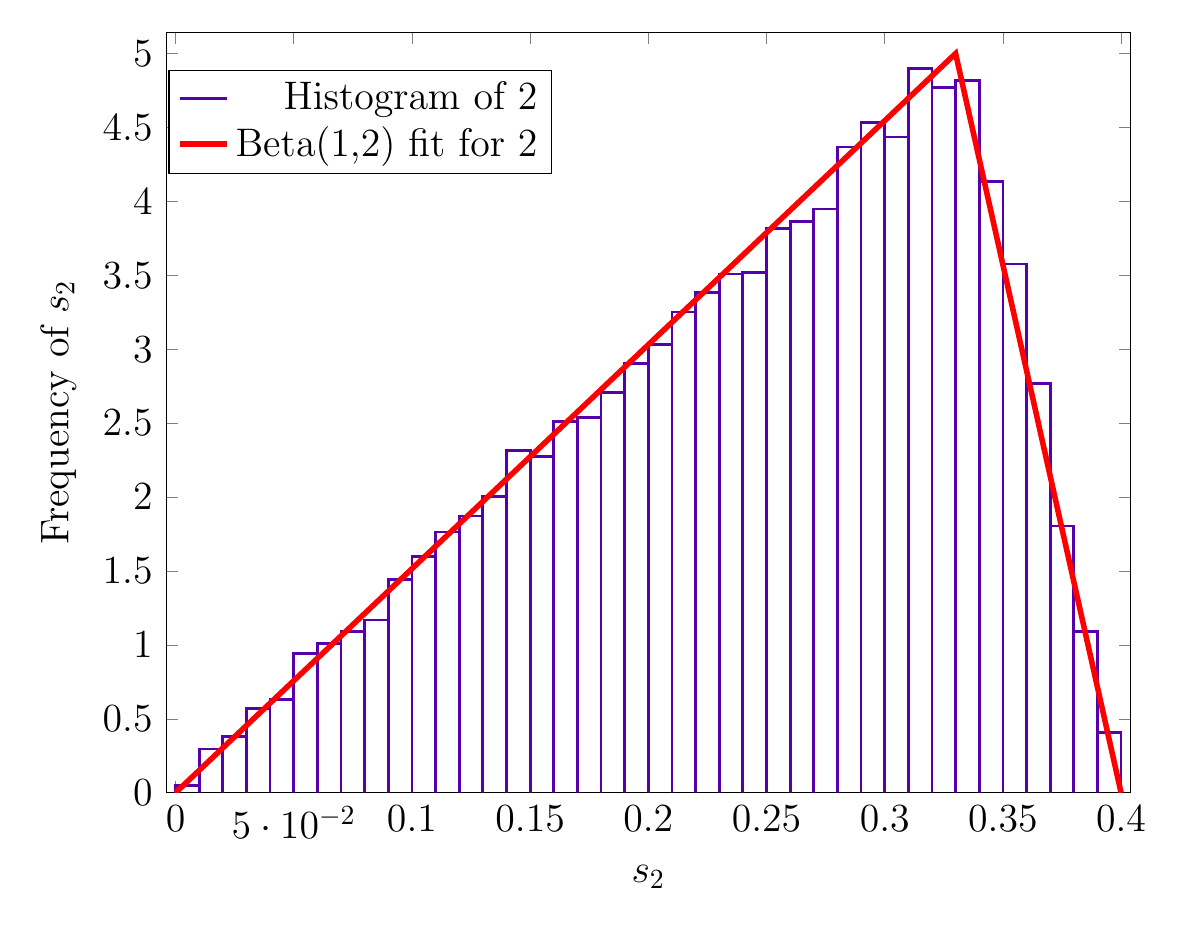
\begin{tikzpicture}
\tikzset{every picture/.style={font issue=\Large},
         font issue/.style={execute at begin picture={#1\selectfont}}
        }
\begin{axis}[%
width=4.82222222222222in,
height=3.80333333333333in,
scale only axis,
xmin=-0.004,
xmax=0.404,
xlabel={$s_2$},
ymin=0,
ymax=5.14499999999889,
ylabel={Frequency of $s_2$},
legend style={draw=black,fill=white,legend cell align=right,at={(.4,0.95)}}
]
\addplot [color=mycolor1,solid,line width=1.0pt]
  table[row sep=crcr]{%
0	0\\
0	0.0480000000000258\\
0.01	0.0480000000000258\\
0.01	0\\
0.01	0\\
0.01	0.296000000000052\\
0.02	0.296000000000052\\
0.02	0\\
0.02	0\\
0.02	0.380000000000013\\
0.03	0.380000000000013\\
0.03	0\\
0.03	0\\
0.03	0.572000000000006\\
0.04	0.572000000000006\\
0.04	0\\
0.04	0\\
0.04	0.631999999999844\\
0.05	0.631999999999844\\
0.05	0\\
0.05	0\\
0.05	0.939999999999984\\
0.06	0.939999999999984\\
0.06	0\\
0.06	0\\
0.06	1.00800000000008\\
0.07	1.00800000000008\\
0.07	0\\
0.07	0\\
0.07	1.09199999999997\\
0.08	1.09199999999997\\
0.08	0\\
0.08	0\\
0.08	1.16800000000011\\
0.09	1.16800000000011\\
0.09	0\\
0.09	0\\
0.09	1.44400000000023\\
0.1	1.44400000000023\\
0.1	0\\
0.1	0\\
0.1	1.60000000000022\\
0.11	1.60000000000022\\
0.11	0\\
0.11	0\\
0.11	1.76400000000001\\
0.12	1.76400000000001\\
0.12	0\\
0.12	0\\
0.12	1.87200000000021\\
0.13	1.87200000000021\\
0.13	0\\
0.13	0\\
0.13	2.0040000000003\\
0.14	2.0040000000003\\
0.14	0\\
0.14	0\\
0.14	2.31600000000018\\
0.15	2.31600000000018\\
0.15	0\\
0.15	0\\
0.15	2.27200000000025\\
0.16	2.27200000000025\\
0.16	0\\
0.16	0\\
0.16	2.51200000000021\\
0.17	2.51200000000021\\
0.17	0\\
0.17	0\\
0.17	2.54000000000047\\
0.18	2.54000000000047\\
0.18	0\\
0.18	0\\
0.18	2.70800000000044\\
0.19	2.70800000000044\\
0.19	0\\
0.19	0\\
0.19	2.90400000000024\\
0.2	2.90400000000024\\
0.2	0\\
0.2	0\\
0.2	3.03200000000059\\
0.21	3.03200000000059\\
0.21	0\\
0.21	0\\
0.21	3.25200000000063\\
0.22	3.25200000000063\\
0.22	0\\
0.22	0\\
0.22	3.38400000000055\\
0.23	3.38400000000055\\
0.23	0\\
0.23	0\\
0.23	3.50800000000022\\
0.24	3.50800000000022\\
0.24	0\\
0.24	0\\
0.24	3.52000000000068\\
0.25	3.52000000000068\\
0.25	0\\
0.25	0\\
0.25	3.8160000000007\\
0.26	3.8160000000007\\
0.26	0\\
0.26	0\\
0.26	3.86399999999946\\
0.27	3.86399999999946\\
0.27	0\\
0.27	0\\
0.27	3.94799999999922\\
0.28	3.94799999999922\\
0.28	0\\
0.28	0\\
0.28	4.36799999999902\\
0.29	4.36799999999902\\
0.29	0\\
0.29	0\\
0.29	4.53199999999877\\
0.3	4.53199999999877\\
0.3	0\\
0.3	0\\
0.3	4.43599999999859\\
0.31	4.43599999999859\\
0.31	0\\
0.31	0\\
0.31	4.89999999999895\\
0.32	4.89999999999895\\
0.32	0\\
0.32	0\\
0.32	4.76800000000003\\
0.33	4.76800000000003\\
0.33	0\\
0.33	0\\
0.33	4.82000000000006\\
0.34	4.82000000000006\\
0.34	0\\
0.34	0\\
0.34	4.13199999999989\\
0.35	4.13199999999989\\
0.35	0\\
0.35	0\\
0.35	3.57599999999987\\
0.36	3.57599999999987\\
0.36	0\\
0.36	0\\
0.36	2.76799999999992\\
0.37	2.76799999999992\\
0.37	0\\
0.37	0\\
0.37	1.80399999999998\\
0.38	1.80399999999998\\
0.38	0\\
0.38	0\\
0.38	1.092\\
0.39	1.092\\
0.39	0\\
0.39	0\\
0.39	0.408000000000008\\
0.4	0.408000000000008\\
0.4	0\\
};
\addlegendentry{Histogram of $\rvsla{2}$};
\addplot [color=red,solid,line width=2.0pt]
  table[row sep=crcr]
{
0  0 \\
0.33 5 \\
0.4 0 \\
};
\addlegendentry{Beta(1,2) fit for $\rvsla{2}$};
  
\end{axis}
\end{tikzpicture}%
}
\end{minipage}
\caption{Histogram of $\rvsla{2}$ restricted to $\Pyr{1}$ for the problem instance $Q = (s=1,n=2,\delta=0,\sat=0.6)$ whose favourable region is the hexagon of \autoref{fig:larged} \cite{KumarTRO15}.}
\label{fig:s2OverP1}
\end{figure} 